% \documentclass[10pt]{sosp2015}
% \documentclass[10pt,onecolumn]{sosp2015}
\documentclass[10pt,onecolumn,letterpaper]{article}
% \usepackage[10pt,inchmargins]{sigmin}  %% template from Xi Wang.
%\special{papersize=8.5in,11in}
%\setlength{\pdfpagewidth}{8.5in}
%\setlength{\pdfpageheight}{11in}
\usepackage[noheadfoot,
	      left=1in,right=1in,top=1in,bottom=1in,
             columnsep=0.3in
             ]{geometry}
\usepackage[small,compact]{titlesec}
\usepackage[font={small,bf}]{caption}    % added 9/10/13
\usepackage[nolineno,noindent,norules]{lgrind}
\usepackage{tightenum}
\usepackage{float}
\usepackage{xspace}
\usepackage{times,pifont}
\usepackage{mathptmx}
\usepackage{subfig,graphics,graphicx,color}
\usepackage{multirow}
\usepackage{dblfloatfix} %% correctly orders single- and double-col figures
\usepackage{hyphenat}
\usepackage{mathrsfs}
\usepackage{subfig}
\usepackage{amssymb,amsmath,centernot}
\usepackage{lastpage}
\usepackage{flushend}
\usepackage{hhline}
\usepackage{authblk}
%\newcommand{\doi}{XXXXXX}


%%% ================= START of SOSP '13 template ================= 
% \makeatletter
% 
% \def\ftype@copyrightbox{8}
% \def\@copyrightspace{
% \@float{copyrightbox}[b]
% \begin{center}
% \setlength{\unitlength}{1pc}
% \begin{picture}(20,6.0) 
% \put(0,3){\parbox{\columnwidth}{\scriptsize
% 
% %*** SAMPLE. AUTHOR PUT SUPPLIED TEXT HERE ****
% 
% \noindent
% \rule{6.0 cm}{0.2pt}\\
% Permissiondddd to make digital or hard copies of part or all of this work 
% for personal or classroom use is granted without fee provided that
% copies are not made or distributed for profit or commercial advantage 
% and that copies bear this notice and the full citation on the first
% page. Copyrights for third-party components of this work must be
% honored.  For all other uses, contact the Owner/Author. 
% 
% \vspace{\baselineskip}\noindent
% Copyright is held by the Owner/Author(s).\\
% \textit{SOSP'15}.\\
% ACM XXXXXXX.
% 
% \noindent
% http://dx.doi.org/\doi}
% }
% \end{picture}
% \end{center}
% \end@float}
% 
% \def\maketitle{\par
%  \begingroup
%    \def\thefootnote{\fnsymbol{footnote}}
%    \def\@makefnmark{\hbox
%        to 0pt{$^{\@thefnmark}$\hss}}
%      \twocolumn[\@maketitle]
% \@thanks
%  \endgroup
%  \setcounter{footnote}{0}
%  \let\maketitle\relax
%  \let\@maketitle\relax
%  \gdef\@thanks{}\gdef\@author{}\gdef\@title{}\gdef\@subtitle{}\let\thanks\relax
%  \@copyrightspace}
% 
% \makeatother

%%% ================= END of SOSP '13 template ================= 



%\newcommand{\comment}[1]{}
\frenchspacing

%\doublespacing

%%%%%%%%%%%%%%%%%%%%%%%%%%%%
%     macro

\newcommand{\xxx}[0]{\textsc{Crane}\xspace}
\newcommand{\paxos}[0]{\textsc{Paxos}\xspace}
\newcommand{\mytitle}[0]{\textbf {Making Threads More Reliabile and Secure 
through Stable Multithreading}}
\newcommand{\mykeywords}[0]{State Machine Replication, Fault Tolerance, Stable 
and Deterministic Multithreading, Software Reliability}

%%%%%%%%%%%%%%%%%%%%%%%%%%%%%%%%%%%%%%%%%%%%%%%%%%%%%%%%%%%%%%%%%
% hyperref stuff

%\usepackage[square,comma,numbers,sort]{natbib}
\usepackage{hypernat}
\usepackage{hyperref}

%% fill in pdf info here
\hypersetup{%
colorlinks=false,
pdfborder={0 0 0},
pdftitle={\mytitle},
pdfkeywords={\mykeywords},
bookmarksnumbered,
pdfstartview={FitH},
urlcolor=cyan,
pdfpagelabels=true,
pdfdisplaydoctitle=true,
}%

%\usepackage{breakurl}
%\usepackage[all]{hypcap}
%\renewcommand{\url}{\burl}

%%%%%%%%%%%%%%%%%%%%%%%%%%%%%%%%%%%%%%%%%%%%%%%%%%%%%%%%%%%%
% Some NICE fonts

\newfont{\BIG}{cminch}                             %--- One-inch font
\newfont{\sfbHuge}{cmssbx10 scaled\magstep5}       %-- 25pt sans serif bold
\newfont{\sfbLarger}{cmssbx10 scaled\magstep3}   %-- 12+pt sans serif boldd
\newfont{\sfblarger}{cmssbx10 scaled\magstep2}   %-- 12+pt sans serif bold
\newfont{\sfblarge}{cmssbx10 scaled\magstep1}      %-- 12pt sans serif bold
\newfont{\sfbeleven}{cmssbx10 scaled\magstephalf}  %-- 11pt sans serif bold
\newfont{\sfb}{cmssbx10}                           %-- 10pt sans serif bold
\newfont{\sfeight}{cmss8}                          %-- 8pt sans serif

%%%%%%%%%%%%%%%%%%%%%%%%
%    space tweaking

%\textwidth = 6.5 in
%\textheight = 9.0 in
%\setlength{\topmargin}{-.5in}

%\headheight = 0.0 in
%\headsep = 0.0 in
%\parskip = 0.2in
%\parindent = 0.0in

\renewcommand{\topfraction}{0.95}
\addtolength{\textfloatsep}{-0.1in}
%\addtolength{\floatsep}{0.025in}
\renewcommand\floatpagefraction{.9}
%\renewcommand\bottomfraction{.9}
\renewcommand\textfraction{.1}

\setlength{\parindent}{9pt}

% Rescue
\makeatletter
\def\v#1{{\mbox{\fontfamily{cmtt}\fontsize{\f@size}{\f@size}\selectfont #1}}}

\newcommand{\dmt}[0]{DMT\xspace}
\newcommand{\smt}[0]{StableMT\xspace}
\newcommand{\smr}[0]{SMR\xspace}

\newcommand{\racepro}[0]{\textsc{RacePro}\xspace}
\newcommand{\criu}[0]{\textsc{CRIU}\xspace}
\newcommand{\lxc}[0]{\textsc{LXC}\xspace}
\newcommand{\tern}[0]{\textsc{Tern}\xspace}
\newcommand{\peregrine}[0]{\textsc{Peregrine}\xspace}
\newcommand{\parrot}[0]{\textsc{Parrot}\xspace}
\newcommand{\repframe}[0]{\textsc{RepFrame}\xspace}
\newcommand{\grace}[0]{Grace\xspace}
\newcommand{\coredet}[0]{\textsc{CoreDet}\xspace}
\newcommand{\kendo}[0]{Kendo\xspace}
\newcommand{\dthreads}[0]{\textsc{DThreads}\xspace}
\newcommand{\determinator}[0]{Determinator\xspace}
\newcommand{\dos}[0]{dOS\xspace}
\newcommand{\ddos}[0]{DDOS\xspace}
\newcommand{\timealgo}[0]{time bubbling\xspace}
\newcommand{\ldpreload}[0]{LD\_PRELOAD\xspace}
\newcommand{\ntimeout}[0]{$W_{timeout}$\xspace}
\newcommand{\nclock}[0]{$N_{clock}$\xspace}

\newcommand{\apache}{\v{Apache}\xspace}
\newcommand{\mongoose}[0]{\v{Mongoose}\xspace}
\newcommand{\ab}{\v{ApacheBench}\xspace}
\newcommand{\clamav}{\v{ClamAV}\xspace}
\newcommand{\upnp}{uPnP\xspace}
\newcommand{\mediatomb}{\v{MediaTomb}\xspace}
\newcommand{\mencoder}{\v{mencoder}\xspace}
\newcommand{\mongodb}{\v{MongoDB}\xspace}
\newcommand{\ssdb}{\v{SSDB}\xspace}
\newcommand{\mysql}{\v{MySQL}\xspace}
\newcommand{\sysbench}{\v{SysBench}\xspace}
\newcommand{\zookeeper}{\v{ZooKeeper}\xspace}


\newcommand{\aget}[0]{\v{aget}\xspace}
\newcommand{\pthread}[0]{\mbox{Pthreads}\xspace}
\newcommand{\openldap}[0]{{OpenLDAP}\xspace}
\newcommand{\redis}[0]{{Redis}\xspace}
\newcommand{\bdb}[0]{{Berkeley DB}\xspace}
\newcommand{\vtune}[0]{\v{VTune}\xspace}
\newcommand{\http}[0]{\mbox{HTTP}\xspace}

% In short.
\newcommand{\eg}{{e.g.}}
\newcommand{\ie}{{i.e.}}
\newcommand{\etc}{{etc}}
\newcommand{\para}[1]{\vspace{.00in}\noindent{\bf #1}}
\newcommand{\wrt}{{w.r.t. }}
\newcommand{\cf}{{cf. }}

% Synch and network operations.
\newcommand{\checktimebubble}[0]{\v{check\_add\_timebubble()}\xspace}
\newcommand{\mutexlock}[0]{\v{pthread\_mutex\_lock()}\xspace}
\newcommand{\connect}[0]{\v{connect()}\xspace}
\newcommand{\send}[0]{\v{send()}\xspace}
\newcommand{\sendto}[0]{\v{sendto()}\xspace}
\newcommand{\sendmsg}[0]{\v{sendmsg()}\xspace}
\newcommand{\mywrite}[0]{\v{write()}\xspace}
\newcommand{\pwrite}[0]{\v{pwrite()}\xspace}
\newcommand{\close}[0]{\v{close()}\xspace}
\newcommand{\recv}[0]{\v{recv()}\xspace}
\newcommand{\select}[0]{\v{select()}\xspace}
\newcommand{\poll}[0]{\v{poll()}\xspace}
\newcommand{\epollwait}[0]{\v{epoll\_wait()}\xspace}
\newcommand{\accept}[0]{\v{accept()}\xspace}

% Parrot primitives.
\newcommand{\getturn}[0]{\v{get\_turn()}\xspace}
\newcommand{\putturn}[0]{\v{put\_turn()}\xspace}
\newcommand{\wait}[0]{\v{wait()}\xspace}
\newcommand{\signal}[0]{\v{signal()}\xspace}

% Evaluation stats.
\newcommand{\github}[0]{\url{github.com/columbia/crane}}
% \newcommand{\ntype}[0]{four\xspace}
\newcommand{\nprog}[0]{five\xspace}
\newcommand{\overheadmax}[0]{22.99\%\xspace}
\newcommand{\overhead}[0]{34.19\%\xspace}
\newcommand{\dmtspeedup}[0]{10.5\%\xspace}
\newcommand{\proxyoverhead}[0]{2.33\%\xspace}
\newcommand{\timebubblelow}[0]{66.65\%\xspace}
\newcommand{\timebubblehigh}[0]{93.88\%\xspace}
\newcommand{\recovertime}[0]{1.97ms\xspace}
\newcommand{\downgradetime}[0]{0.36s\xspace}
\newcommand{\mencoderspeedup}{\v{49\%}\xspace}

\def\LGfsize{\footnotesize}
%\pagestyle{empty}


% \conferenceinfo{SOSP'15}{October 4--7, 2015, Monterey, CA}
% \copyrightyear{2015} 
% \copyrightdata{978-1-4503-3834-9/15/10} 
% \doi{2815400.2815427}

\title{\mytitle}
% \authorinfo{Authors}

% \author[+*]{Heming Cui}
% \author[*]{Rui Gu}
% \author[*]{Cheng Liu}
% \author[x]{Tianyu Chen}
% \author[*]{Junfeng Yang}
% \setlength{\affilsep}{0.5em}
% \renewcommand\AB@affilsepx{\hspace{28.0 mm}\protect\Affilfont}
% \affil[+]{\textrm\fontsize{10}{10}\selectfont The University of Hong Kong}
% \affil[*]{\textrm Columbia University}
% \affil[x]{\textrm Tsinghua University\vspace{-7.0 mm}}

\begin{document}

% Hack for: Package caption Error: No float type 'copyrightbox' defined.
%\newcounter{copyrightbox}

\date{}

\author[+]{Authors}
\maketitle
%\thispagestyle{empty}

% \begin{sloppypar}
% \begin{abstract}
% \input{abstract}
% \end{abstract}
% \end{sloppypar}

% \begin{sloppypar}
%% %\category{D.2.5}{Software Engineering}{Testing and Debugging}
%% \category{D.4.5}{Operating Systems}{Threads, Reliability}
%% \category{D.2.4}{Software Engineering}{Software/Program Verification}
%% \terms{Algorithms, Design, Reliability, Performance}
%% \keywords{\mykeywords}

%% \vskip 2mm
%% \noindent {\small \bf Categories and Subject Descriptors:} \vskip -.2mm
%% \noindent
%% {\footnotesize D.4.5~[{\bf Operating Systems}]: {Threads, Reliability}\\
%% D.2.4~[{\bf Software Engineering}]: {Software/Program Verification};}
%% \vskip 1mm
%% \noindent {\small \bf General Terms:} \vskip -.2mm
%% \noindent
%% {\footnotesize Algorithms, Design, Reliability, Performance}
%% \vskip 1mm
%% \noindent {\small \bf Keywords:} \vskip -.2mm
%% \noindent
%% {\footnotesize \mykeywords}

% \vskip 2mm
% \noindent {\small \bf Categories and Subject Descriptors:}
% {\small D.4.5~[{\bf Operating Systems}]: {Threads, Reliability};
%   D.2.4~[{\bf Software Engineering}]: {Software/Program Verification};}
% \vskip .1mm
% \noindent {\small \bf General Terms:} {\small Algorithms, Design,
%   Reliability, Performance}
% \vskip .1mm
% \noindent {\small \bf Keywords:} {\small \mykeywords}
% 
% \end{sloppypar}

%%%%%%%%%%%%%%%%%%%%%%%%%%%%%%%%%%%
% Add page number.
\setcounter{page}{1}
\pagenumbering{arabic}

\thispagestyle{plain}
\pagestyle{plain}
\setlength{\footskip}{20pt}
%%%%%%%%%%%%%%%%%%%%%%%%%%%%%%%%%%%

% \begin{sloppypar}
% 
% \vskip 2mm
% \noindent {\small \bf Categories and Subject Descriptors:}
% {\small D.4.5~[{\bf Operating Systems}]: {Threads, Reliability};
%   C.2.4~[{\bf Computer-communication Networks}]: {Distributed Systems};}
% \vskip .1mm
% \noindent {\small \bf General Terms:} {\small Algorithms, Design,
%   Reliability, Performance}
% \vskip .1mm
% \noindent {\small \bf Keywords:} {\small \mykeywords}
% 
% \end{sloppypar}

\begin{sloppypar}

Multithreaded programs have become pervasive due to the accelerating  
computational demand and the rise of multi-core hardware. Unfortunately, despite 
much research and engineering effort, these programs are still notoriously 
difficult to get right. They are plagued with concurrency bugs, which can easily 
cause severe program behaviors such as wrong outputs, program crashes, and 
security breaches.

Our research~\cite{smt:cacm} reveals that a key reason of this difficulty is 
that  multithreaded programs have too many possible thread interleavings, or 
schedules. Even given only a single input, a program may run into excessive 
schedules, depending on factors such as hardware timing and OS scheduling. 
Considering all inputs, the number of schedules is even much greater. Finding a 
buggy schedule in this huge schedule set is like finding a needle in a haystack, 
which aggravates understanding, testing, and analyzing of programs. For 
instance, testing is ineffective because the schedules tested in the lab may not 
be the ones run in the field.

To reduce the number of schedules for all inputs, we have studied the relation  
between inputs and schedules of real-world programs, and made a surprising 
discovery: many programs require only a small set of schedules to efficiently 
process a wide range of inputs. Leveraging this discovery, we have proposed the 
idea of stable multithreading (StableMT) [5] that reuses each schedule on a wide 
range of inputs. StableMT conceptually maps all inputs to a greatly reduced set 
of schedules, drastically shrinking the “haystack”, making the “needles” much 
easier to find. StableMT can greatly benefit understanding multithreaded 
programs and many reliability techniques, including testing, debugging, 
replication, and verification. For instance, testing schedules in such a much 
smaller schedule set becomes a lot more effective.

StableMT is complementary to another idea called deterministic multi-threading  
(DMT) that enforces the same schedule on each input. Our 
research~\cite{smt:cacm} has shown that although DMT is useful, it is not as 
useful as commonly perceived, because a DMT system can map slightly changed 
inputs to very different schedules, which can easily cause very different 
program behaviors. Furthermore, the number of schedules for all inputs in DMT 
can still be extremely large, which is the key problem that StableMT mitigates. 


\begin{figure*}[ht]
\begin{center}
\subfloat[{\em
Traditional.}]{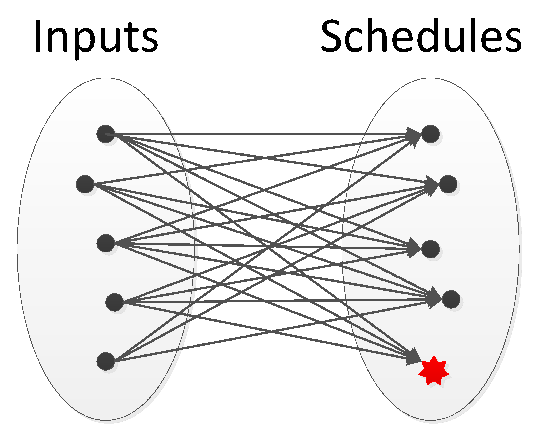
\includegraphics[width=.23\linewidth]{figures/nondet}
  \label{fig:nondet}}
\subfloat[{\em
Deterministic.}]{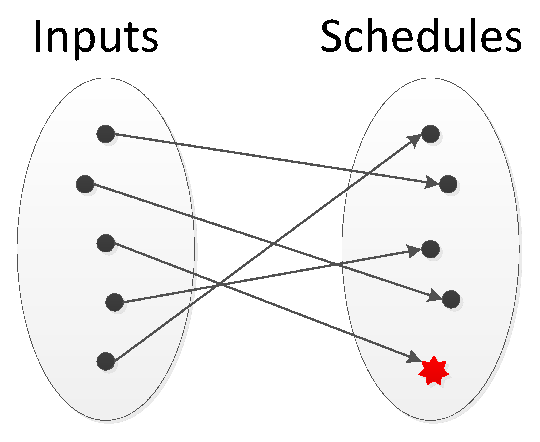
\includegraphics[width=.23\linewidth]{figures/dmt}
  \label{fig:dmt}}
\subfloat[{\em Stable
(deterministic).}]{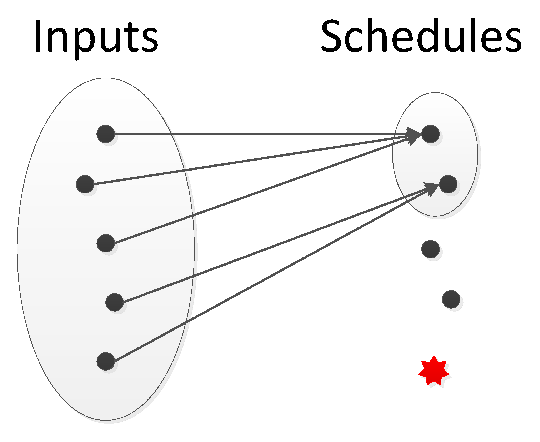
\includegraphics[width=.23\linewidth]{figures/smt}
  \label{fig:smt}}
\subfloat[{\em Stable
(nondeterministic).}]{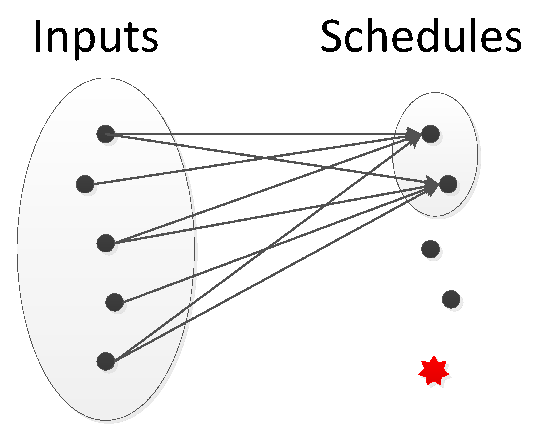
\includegraphics[width=.23\linewidth]{figures/smtn}
  \label{fig:smtn}}
\vspace{-.05in}
\caption{Different multithreading approaches. Red stars represent buggy
schedules.}\label{fig:compare}
\vspace{-.2in}
\end{center}
\end{figure*}

Figure~\ref{fig:compare} shows different multithreading 
approaches in a conceptual level. Traditional multithreading 
(Figure~\ref{fig:nondet}) is a conceptual many-to-many mapping between inputs 
and schedules.  \dmt (Figure~\ref{fig:dmt}) may map each input to an arbitrary 
schedule, reducing programs' robustness on input perturbations.  \smt 
(Figure~\ref{fig:smt} and Figure~\ref{fig:smtn}) reduces the total set of 
schedules for all inputs (represented by the shrunk ellipses), increasing 
robustness and improving reliability. \smt is complementary to \dmt: a \smt 
system can be deterministic (Figure~\ref{fig:smt}) or nondeterministic 
(Figure~\ref{fig:smtn}). Notably, StableMT has attracted the research 
community’s interest since it was 
initially proposed by us~\cite{cui:tern:osdi10}, and most subsequent systems 
are both StableMT and DMT.

To realize StableMT, we have built three systems, \tern~\cite{cui:tern:osdi10}, 
\peregrine~\cite{peregrine:sosp11},  and \parrot~\cite{parrot:sosp13}, with 
each addressing a distinct challenge. Moreover, to justify the benefits of 
StableMT, we have applied StableMT to several reliability and security 
topics, including improving precision of static analysis~\cite{wu:pldi12}, 
detecting security rule violations~\cite{woodpecker:asplos13}, and building 
transparent state machine replication service for general multithreaded 
programs~\cite{crane:sosp15}.

\end{sloppypar}

% uncomment to tweak with bib spacing
%\setlength\bibsep{2.25pt}
{
%\small
 \bibliographystyle{abbrv}
 \bibliography{bib/biblio}
}

\end{document}
